% =====================================================================
% Avaliação de desempenho --- Iago (Frente 3)
% Só o Iago edita este arquivo. Os números vêm de desempenho/resultados/.
% =====================================================================
\section{Avaliação de desempenho}\label{sec:desempenho}

Para verificar se as complexidades se confirmam na prática e quanto custa o Python puro, medimos as
centralidades da Seção~\ref{sec:centralidades} e a busca em largura (BFS) com o nosso código e com o
NetworkX 3.7~\cite{hagberg2008}, que o enunciado só permite usar nesta comparação. Os scripts e os
resultados completos ficam em \codigo{desempenho/}.

\paragraph{Metodologia.} Usamos grafos de Erdős--Rényi, Barabási--Albert e Watts--Strogatz
($p = 0{,}1$) com 1.000 a 100.000 nós, grau médio 10 e semente 42, além das quatro bases. O tempo é a
mediana de 5 execuções com \codigo{time.perf\_counter}, e o pico de memória é o que a função aloca
durante a chamada, medido com \codigo{tracemalloc}; na BFS, medimos também as arestas percorridas por
segundo (TEPS). No NetworkX, o PageRank é a versão em Python puro, porque a padrão depende do SciPy.
A intermediação exata, de custo $O(nm)$, só foi medida até 5.000 nós, em que já leva cerca de
20~s; acima disso, só a amostrada, com $k = 100$. As medições rodaram num AMD Ryzen 5 7600X com
14,7~GiB de RAM, Ubuntu 24.04 e Python 3.12.3.

\begin{figure}[tb]
\centering
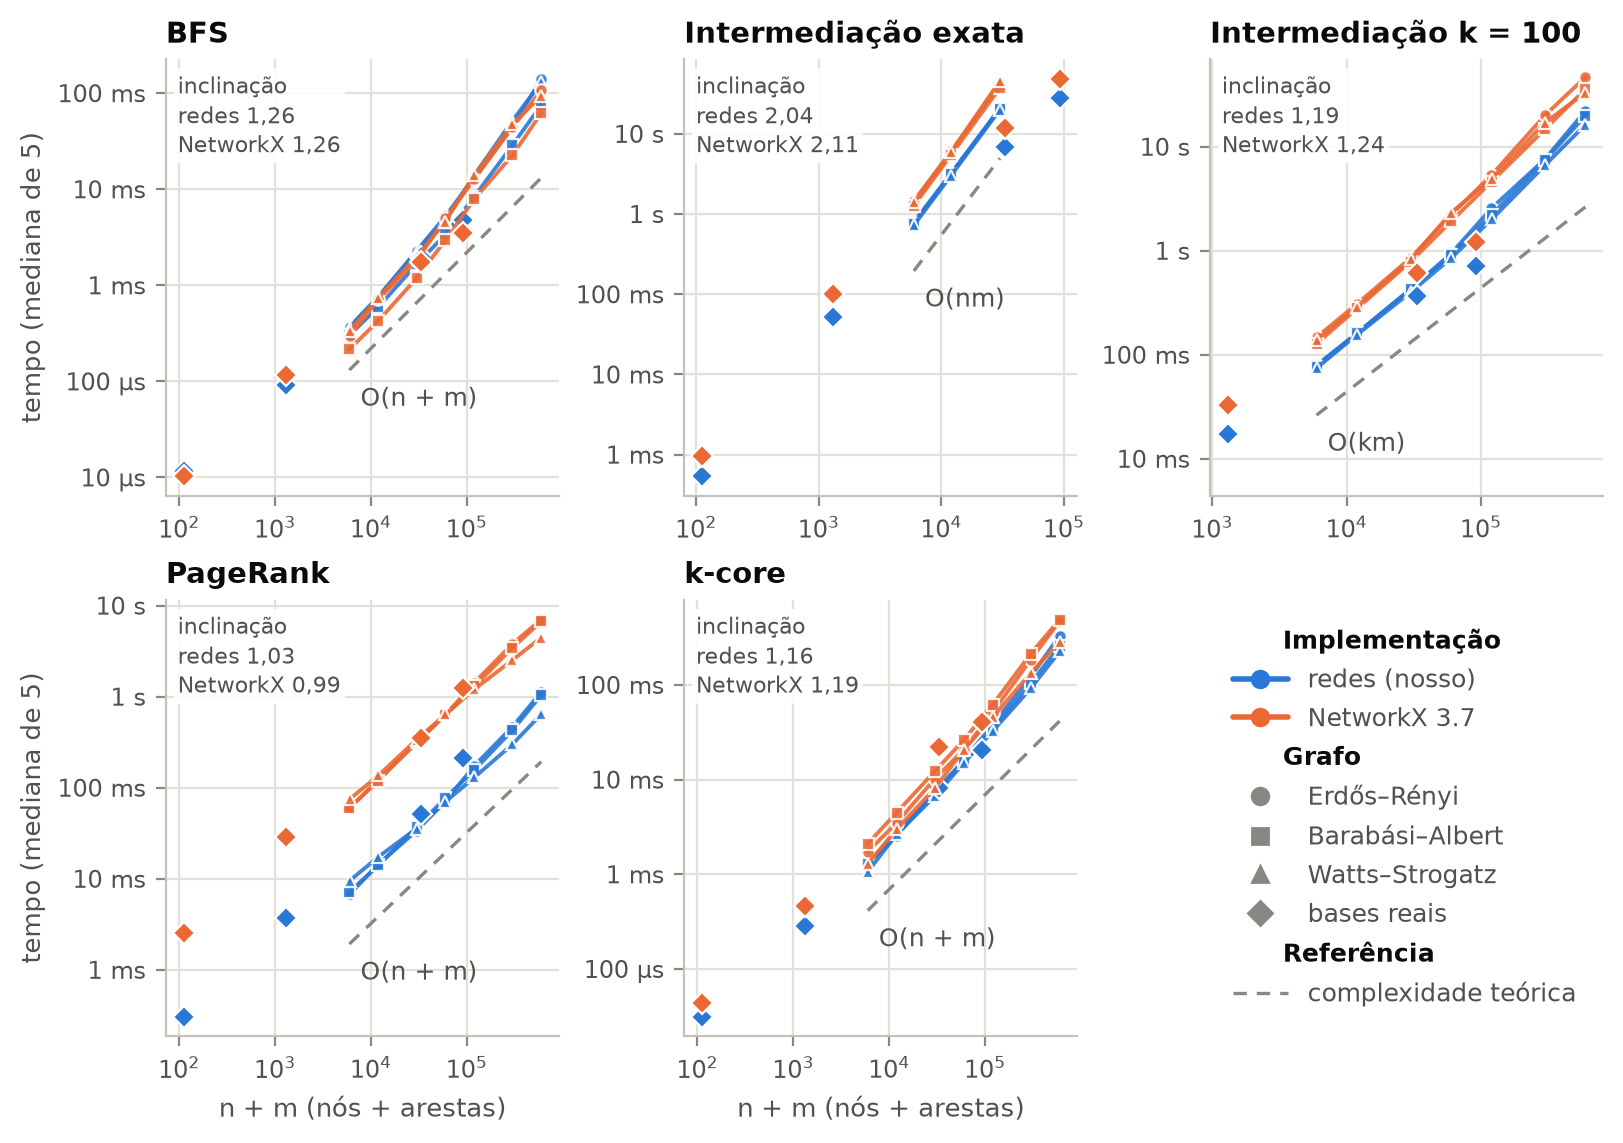
\includegraphics[width=.7\textwidth]{tempo_loglog.png}
\caption{Tempo (mediana de 5 execuções) em função de $n + m$, em escala log-log. Azul: nosso
código; laranja: NetworkX 3.7. As linhas são os grafos sintéticos, os losangos, as quatro bases, e o
tracejado, a complexidade teórica, deslocada para baixo.}
\label{fig:tempo-loglog}
\end{figure}

\begin{table}[tb]
\centering
\caption{Inclinação $b$ do ajuste $\text{tempo} \approx a\,(n + m)^b$ nos grafos sintéticos e
tempo na Twitch PT ($n = 1.912$ e $m = 31.299$). A razão é o tempo do NetworkX dividido pelo nosso:
acima de 1, o nosso código é mais rápido.}
\label{tab:desempenho}
\small
\begin{tabularx}{\textwidth}{@{}Y c c c r r r@{}}
\toprule
& \multicolumn{3}{c}{Inclinação $b$} & \multicolumn{3}{c}{Tempo na Twitch PT} \\
\cmidrule(lr){2-4} \cmidrule(l){5-7}
Algoritmo & Esperada & Nosso & NetworkX & Nosso & NetworkX & Razão \\
\midrule
BFS (uma origem) & 1 & 1,26 & 1,26 & 2,0 ms & 1,7 ms & 0,9 \\
Intermediação exata & 2 & 2,04 & 2,11 & 6,96 s & 11,69 s & 1,7 \\
Intermediação ($k = 100$) & 1 & 1,19 & 1,24 & 364 ms & 611 ms & 1,7 \\
PageRank & 1 & 1,03 & 0,99 & 51,5 ms & 351 ms & 6,8 \\
$k$-core & 1 & 1,16 & 1,19 & 8,1 ms & 21,9 ms & 2,7 \\
\bottomrule
\end{tabularx}
\end{table}

\paragraph{Resultados.} A Figura~\ref{fig:tempo-loglog} e a Tabela~\ref{tab:desempenho} confirmam as
complexidades: a intermediação exata cresce com inclinação próxima de 2, porque, com $m \approx 5n$,
o custo $O(nm)$ cresce como $(n + m)^2$, e os algoritmos lineares em $n + m$ têm inclinação próxima
de 1. O expoente um pouco acima de 1 na BFS, na intermediação amostrada e no $k$-core
vem, provavelmente, da memória cache: o TEPS da BFS cai de 14--17 milhões, com 1.000 nós, para
4--7 milhões, com 100.000. Nos grafos sintéticos
e nas bases (menos o Karate, de tempos muito pequenos), o nosso código foi de 1,7 a 2,7 vezes mais
rápido que o NetworkX na intermediação, de 1,1 a 2,7 vezes no $k$-core e de 6 a 9,5 vezes no
PageRank, e os dois empataram na BFS (de 0,7 a 1,3 vez). A vantagem vem das listas indexadas: o
NetworkX percorre dicionários e, no PageRank, monta antes uma cópia do grafo com os pesos
normalizados, por isso também usa de 5 a 6 vezes mais memória. Nos demais algoritmos, a memória foi
parecida e cresceu linearmente, como esperado para o espaço $O(n + m)$. Com 100.000 nós, a
intermediação amostrada leva cerca de 20~s, e a exata levaria mais de duas horas.
